\chapter[RoBétArmé: Robots for rebar repair and shotcreting]{RoBétArmé: Human-robot collaborative construction system for shotcrete digitization and automation through advanced perception, cognition, mobility and additive manufacturing skills}

\vspace{-1cm}
\minitoc

\section{Summary}

\begin{itemize} \small
  \item Financed by European Union’s Horizon Europe research and innovation programme (GA 101058731) \vspace{-1em}
  \item Centre for Technology and Research Hellas, Thessaloniki, Greece \vspace{-1em}
  \item Duration: 2023/09--2025/11
\end{itemize}

\noindent \textbf{In a nutshell}: \href{https://www.robetarme-project.eu/}{\texttt{[website]}} \href{https://www.linkedin.com/company/robetarmeproject/posts/?feedView=all}{\texttt{[in]}} \href{https://www.youtube.com/@robetarmeproject5652}{\texttt{[videos]}} \texttt{(all code is private I'm afraid)}\\


\begin{figure}[H]\centering
  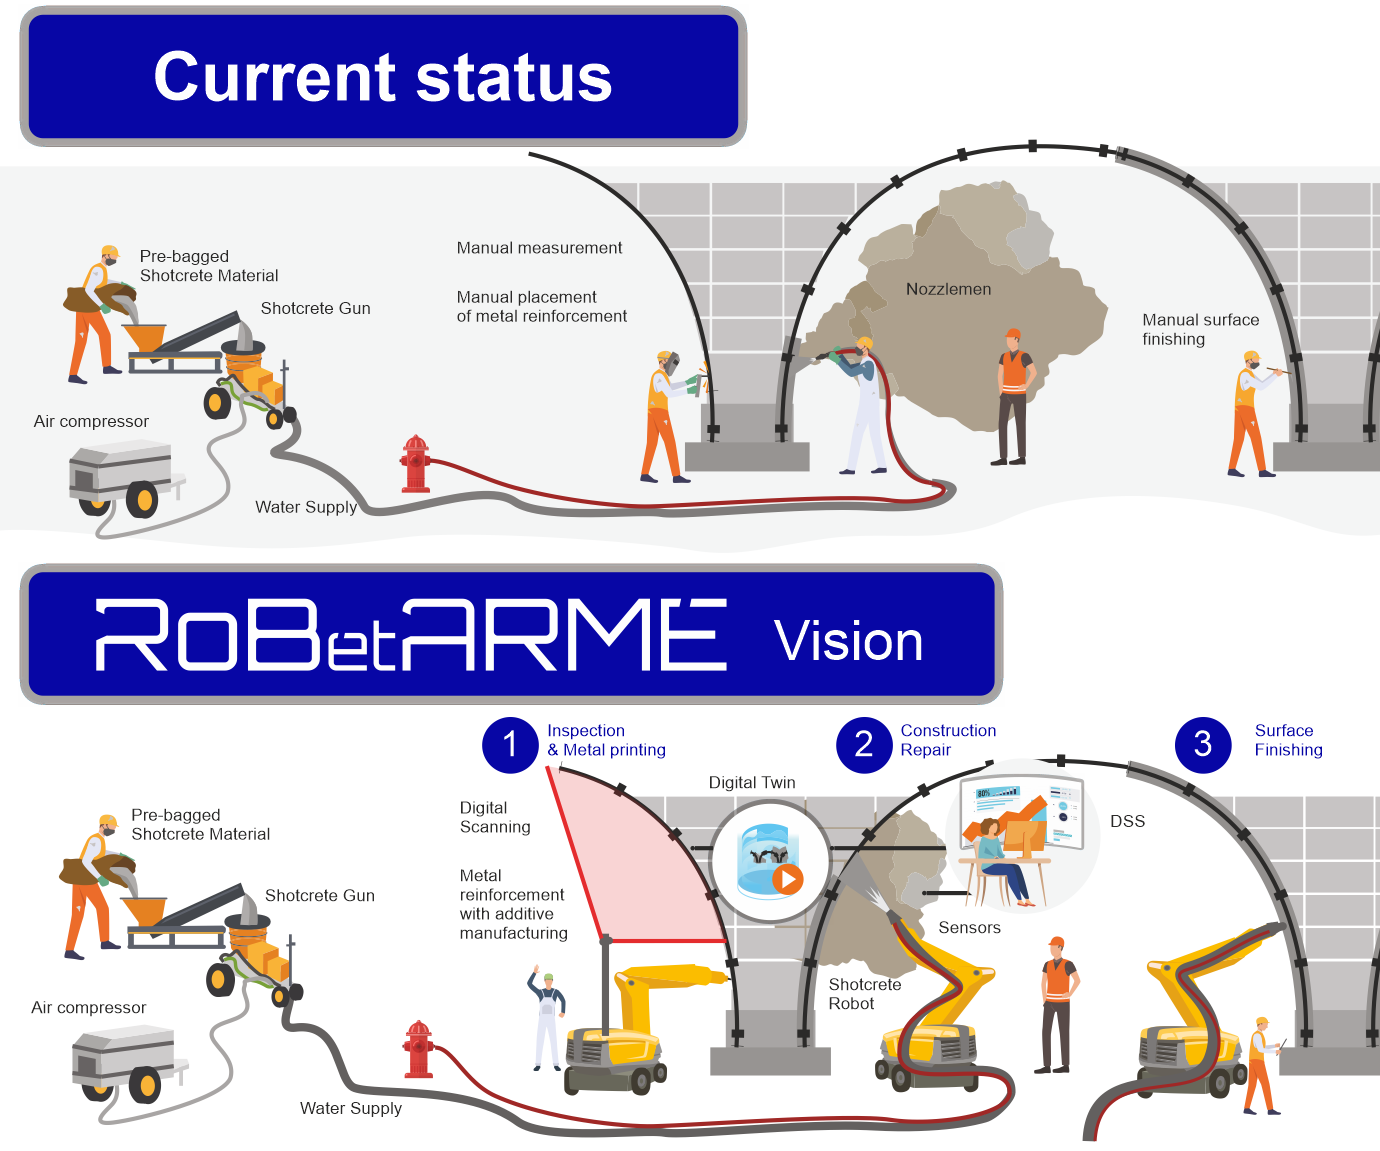
\includegraphics[scale=1.0]{images/robetarme/robetarme_intro.png}
  \caption{\small The project aims to develop automated---standalone or
           assisting---solutions in the construction domain, specifically for
           (a) rebar repair and (b) shotcreting}
  \label{fig:robetarme_intro}
\end{figure}

\textbf{Motivation}: According to the World Economic Forum, the construction
industry accounted for about $6\%$ of the world gross domestic product in
$2022$ and is expected to reach around $14.7\%$ in $2030$. Analogous to
Industry 4.0, breakthrough technologies have been adapted for construction
applications; RoBétArmé aims toward a step-change in Construction 4.0 by
automating laborious tasks in all phases of shotcrete application. To this end
RoBétArmé will deliver collaborative construction mobile manipulators,
consisting of (a) a Inspection Reconnaissance robot (IRR) to address fast, high
precision modeling and rebar reinforcement through metal additive manufacturing
and (b) a Shotcrete and Finishing mobile robot (SFR) to address autonomous
shotcrete application and surface finishing.

\section{My contribution}

In RoBétArmé my contribution was in principle twofold:
\begin{itemize}
  \item I led and executed task \textit{T4.6 - Task Planning and Site Orchestration}
  \item I led and conducted the project's total software integration
\end{itemize}

Specifically, Behaviour Trees\footnote{In C++ via BehaviorTree.CPP:
\url{https://github.com/BehaviorTree/BehaviorTree.CPP}} were used to plan and
order the sequence of events prescribed by the project's use cases. ROS 2
Humble packages for planning tasks in specific machines were then designed.
These had the explicit purpose of interacting between the consortium partners'
own ROS packages and a higher authority called "site orchestrator". The site
orchestrator was executed in a central control unit and had the role of
triggering the task planners specific to computation machines, which in turn
triggered leaf nodes. Subsequently nodes designed to act as templates of nodes
for partners to use as interfaces between task T4.6's task planners and their
own nodes were implemented in \texttt{rclcpp}, \texttt{rclpy}, \texttt{roscpp},
and \texttt{rospy}, thoroughly refined through testing, and then documented
both in a developer's manual manner and for the benefit of the task's own
deliverable report. These and helper packages (e.g. for executing arbitrary
code which is not expressed through ROS) were enclosed in a Docker image where,
during building, lint tests and behaviour trees xml test were held in order to
guarantee execution integrity.

For integration, Docker base images were constructed for ROS noetic, ROS
melodic, and ROS 2 humble, and disseminated to the consortium's partners.
Based on those, template Docker images for the same ROS distributions were also
crafted and disseminated in order for partners to devote more time to the
development of their functionality and less time wrapping it into Docker, as
some we were told were not familiar with Docker. The rationale here is that
since a complete transition to ROS 2 is impossible for some partners, both ROS
versions should be supported.  This also meant that support for interfacing
these two distributions should be offered; this included also the support for
custom interfaces (msgs and srvs---actions are unbridgeable till today). This
effort was arduous and took quite some time, but in the end we were rewarded
with success as well as smoothness due to an eventual refined
\texttt{ros1\_bridge}. Git repositories were set up in GitLab and so were CI/CD
pipelines so that images were immediately built and pushed to a custom
container registry upon pushing of commits. Additionally, since the project
required communications of ROS and ROS 2 nodes between different machines,
Zenoh's \texttt{zenoh-plugin-ros2dds} was utilised, well before
\texttt{rmw\_zenoh} was implemented. In principle the outline of an
architecture encompassing custom communications between nodes of different ROS
versions across multiple machines is exhibited in figure
\ref{fig:robetarme_full_arch_comms}.

\begin{figure}[H]\centering
  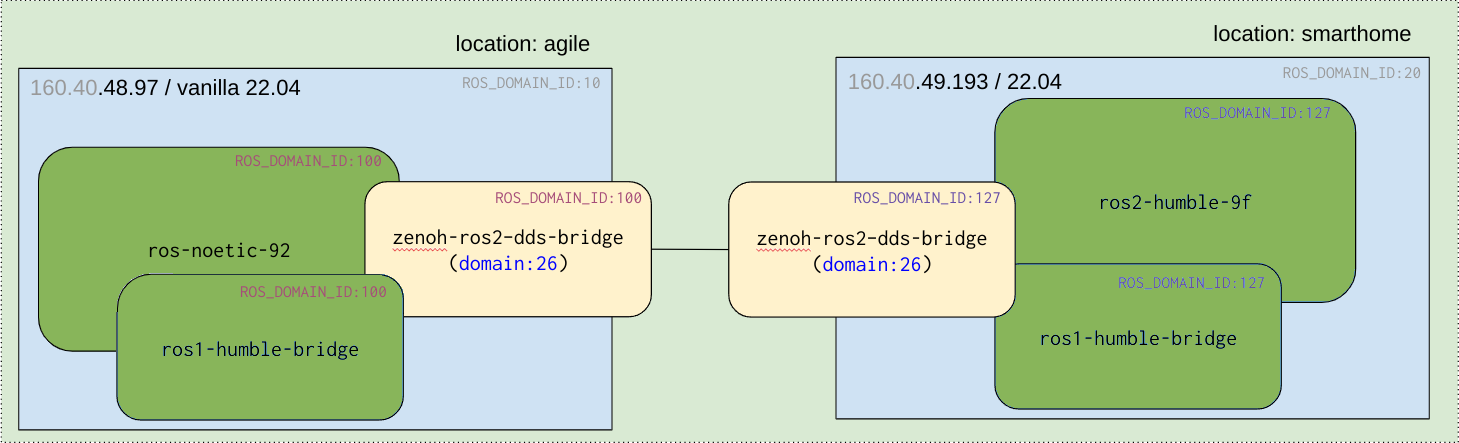
\includegraphics[scale=0.3]{images/robetarme/exp_setup_block.png}
  \caption{\small What the communications architecture looks like when bridging
           ROS nodes of different versions across different machines. In this
           particular example the use of two bridges is superfluous; it is
           necessary though in the general case when ROS nodes of mixed
           versions reside in any single machine.  All boxes with round
           corners signify Docker containers}
  \label{fig:robetarme_full_arch_comms}
\end{figure}

You may find an extensive briefing of all of the project's objectives,
applications, advantages and more at its website:
\url{https://www.robetarme-project.eu/}.

\section{Outcomes}

\begin{itemize}
  \item Notions/resources/tools used: \texttt{ROS melodic} \texttt{ROS noetic},
    \texttt{ROS 2 Humble}, Linux (Ubuntu 20.04 LTS, 22.04 LTS), Docker, Docker compose, Zenoh, OUSTER LIDAR (3D), 2D SLAM (\texttt{slam\_toolbox}, ASTRA, Realsense, ZED2, RC Visard Depth Cameras, SICK visionary-t mini 3D camera,  ROS 2 autonomous navigation stack \texttt{nav2}, \texttt{git}, CI/CD, \texttt{stunnel}
\end{itemize}


\section{Videos of key project aspects}

\begin{itemize}
  \singlespacing
  \item \href{https://www.youtube.com/watch?v=WxfIEvFEOGk}{Premise and motivation introduction}
  \item \href{https://www.youtube.com/watch?v=JWWN4qOTwPs}{2nd Integration Meeting}
\end{itemize}


\section{Details}

There are two pipelines, one for each robot. In the first phase the IRR robot
constructs the 2D map of the construction site and its 3D reconstruction in
mesh form. At the same time the physical space is scanned for openly exposed
rebars, detected via state-of-the-art neural networks tailored for this
purpose.  Once the entire area is surveyed, the areas with concrete defects
(where the exposed rebars show through) are processed as molds, and the volume
to be filled with shotcrete so as to repair them is generated. These volumes
are exported to AR goggles, ready to be further refined by human hand, or new
to be inserted from scratch. Once volumes are settled, the robot now goes into
the second phase, where a trailer carrying additive manufacturing equipment
will have the chance to first repair faulty rebars before them being covered
with shotcrete by the SFR robot. The mobile base plus trailer combination will
travel to each region having concrete defects via autonomous navigation, whose
goals were calculated right after the number and nature of volumes is settled
according to the reach of the manipulator contained within the AM equipment.

In the third phase, after rebars have been repaired, the SFR robot travels
autonomously to the same areas, possibly to new goals depending on the nature
of its own manipulator, and performs the actual shotcreting, after which the
surface is finished as in conventional practice.
